\section{Produit scalaire}

Cette partie présente notre implémentation du produit scalaire sur des vecteurs de flottants à double précision \texttt{ddot}. Dans un premier temps, nous présenterons quel est le problème théorique à résoudre comme définit par la norme BLAS. Ensuite nous verrons comment nous avons implémenté cette routine, et quelles optimisations nous avons tenté de mettre en place. Et enfin nous analyserons les données récoltées lors des \emph{benchmarks}.

\subsection{Problème}

\paragraph{Entrées.} Les entrées sont deux vecteurs $X$ et $Y$ de taille $N$. Chaque vecteur est représenté par les éléments suivants:
\begin{itemize}
\item Un pointeur vers l'adresse du premier élément $X$;
\item Sa taille $N$
\item Le pas $incX$
\end{itemize}
En mémoire, les éléments des vecteurs sont espacés du pas qui définit le vecteur, et peuvent ne pas être contigus en mémoire.

\paragraph{Sortie.} Le résultat de la routine est valeur du produit scalaire:

\begin{equation}
    (X \cdot Y) = \sum\limits_{i=1}^m X_i \cdot Y_i
\end{equation}

\paragraph{Complexité.} On effectue $N$ multiplications et $N-1$ additions flottantes. La complexité de cette routine est:

\begin{equation}
    C(N) = 2N-1
\end{equation}

\subsection{Algorithmes}

Deux algorithmes ont été implémentés pour le produit scalaire \texttt{ddot}: l'algorithme de base, que nous avons ensuite tenté d'optimiser dans le cas ou les vecteurs étaient stockés de manière contiguë.
    
\subsubsection{Algorithme de base}

La première version est une somme par accumulation des multiplications successives sous la forme suivante :
\begin{equation}
    res += X[i*incX]*Y[i*incY]
\end{equation}
$i$ est compris dans l'intervalle allant de 1 à la taille des vecteurs. Nous effectuons alors trois multiplications au lieu d'une seule dans la formule mathématique du produit scalaire, et les deux supplémentaires ne sont nécessaires que pour le parcours des vecteurs dont les éléments ne sont pas contigus.

\subsubsection{Tentative d'optimisation/idées}

L'algorithme général précédent peut être amélioré lorsque $incX = incY = 1$. Les multiplications par $incX$ et $incY$ sont maintenant inutiles et nous pouvons simplifier la formule :
\begin{equation}
    res += X[i]*Y[i]
\end{equation}
Dans ce cas, la localité spatiale est plus importante, et des mécanismes comme le \emph{prefetching} et la vectorialisation sont plus facilement utilisables. Même si les optimisations \texttt{-O2} ne mettent pas en place ces mécanismes, on espère gagner en performances en évitant de faire une multiplication par $incX$ inutile.
    
Une autre optimisation possible serait la parallélisation en découpant les vecteurs en blocs et en distribuant les calculs des produits scalaires des blocs sur différents processeurs.



\subsection{Benchmark}

Nous avons effectué différentes mesures de performances afin d'analyser les routines que nous avons implémenté. Nous avons fait varier la taille des données, mais aussi la distribution des données en mémoire, et avons comparé nos résultats à ceux de MKL.

Pour représenter les données collectées, nous avons effectué 3 graphiques illustrant la performance en fonction de la taille du vecteur que l'on peut voir dans la figure \ref{fig:graph_vec}.
%\begin{enumerate}[label=\alph*.]
%\item 
%\end{enumerate}

\begin{figure}[ht]
\centering
\begin{subfigure}[b]{.5\textwidth}
  \centering
  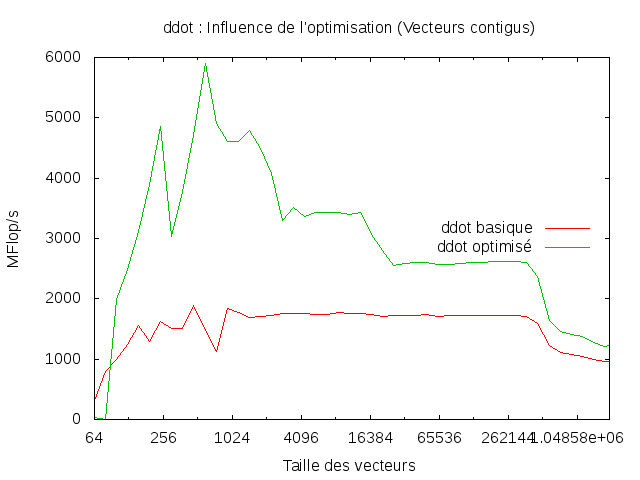
\includegraphics[width=\textwidth]{vec_opt.png}
  \caption{Impact de l'optimisation}
  \label{fig:vec_opt}
\end{subfigure}%
\begin{subfigure}[b]{.5\textwidth}
  \centering
  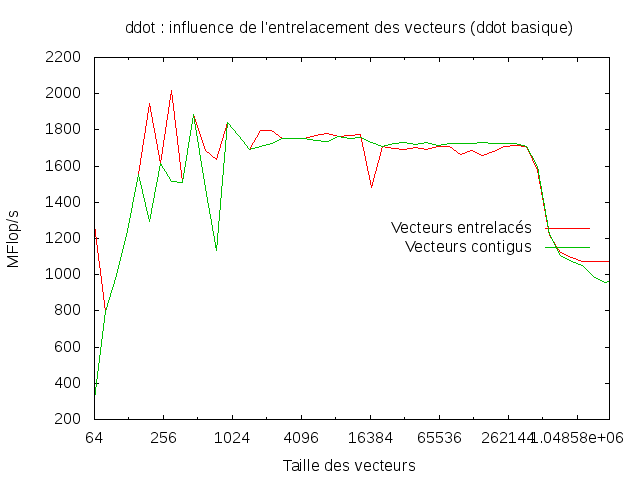
\includegraphics[width=\textwidth]{vec_int.png}
  \caption{Impact de l'entrelacement}
  \label{fig:vec_int}
\end{subfigure}
\begin{subfigure}[b]{.5\textwidth}
  \centering
  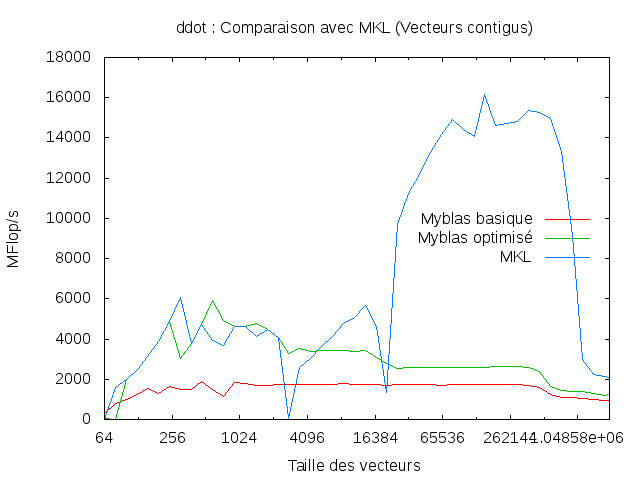
\includegraphics[width=\textwidth]{vec_mkl.png}
  \caption{Comparaison avec MKL}
  \label{fig:vec_mkl}
\end{subfigure}
\caption{Benchmarks pour \texttt{ddot}}
\label{fig:graph_vec}
\end{figure}

La figure \ref{fig:vec_opt} présente les courbes de performances des deux routines implémentées, avec et sans optimisation. 

La figure \ref{fig:vec_int} présente les courbes de performances de notre routine basique selon la distribution des vecteurs en mémoire. On oppose la distribution contiguë ($X_1\cdots X_nY_1\cdots Y_n$) en mémoire à la distribution entrelacée ($X_1Y_1\cdots X_nY_n$). Les autres \emph{benchmarks} sont effectués avec des vecteurs contigus.

La figure \ref{fig:vec_mkl} compare nos algorithmes à la bibliothèque MKL.

\subsubsection{Influence de la taille des vecteurs}

Sur toutes les courbes de la figure \ref{fig:graph_vec}, les performances sont mauvaises lorsque $N$ est très petit ($<100$). Cela est probablement dû aux temps de calculs trop courts qui ne permettent pas de négliger les opération périphériques, telles que les appels de fonctions ou le mécanisme de mesure de temps. Il peut aussi s'agir de l'effet pipeline qui n'intervient que lorsque $N$ est assez grand.
    
On remarque aussi toujours une chute de performances autour de $10^6$, qui se trouve être l'ordre de grandeur du cache L3 (8MB). Dans le même ordre d'idée, sur certaines courbes des creux apparaissent aux alentours de 1000, ce qui est comparable à la taille des caches L1 du processeur (32KB).

\subsubsection{Influence de l'optimisation}

La figure \ref{fig:vec_opt} montre que pour des vecteurs contigus la version optimisée est bien plus rapide que la version basique.
    
Pour $N$ compris entre $10^2$ et $10^4$, les performances sont bien plus élevées, avec une accélération de l'ordre de 4. Entre $10^4$ et $10^6$ le calcul se fait 2 fois plus vite.
    
Le nombre d'opérations de la version optimisée est comparable à la moitié de la fréquence du processeur (2.66GHz). Ceci est probablement du au fait que cet algorithme effectue une multiplication entière pour une opération flottante (2 multiplications pour l'indice, une addition et une multiplication flottante).
    
L'algorithme optimisé donne des valeurs supérieures à la fréquence du processeur entre $10^2$ et $10^4$. Cela indique que plus d'une unité flottante est utilisée à la fois sur le processeur. Il s'agit probablement d'une optimisation impliquant de la vectorialisation par le compilateur intel ou par le matériel. Au delà de $10^4$ on observe un palier dont la valeur est comparable à la fréquence du processeur, ce qui indique qu'un calcul flottant est effectué par cycle. Le gain de performance entre la version optimisée et la version non optimisée semble logique vis-à-vis de la suppression d'une multiplication entière dans la version optimisée.
    
\subsubsection{Influence de l'entrelacement}

La figure \ref{fig:vec_int} montre que les deux distributions de données donnent des résultats similaires pour l'algorithme non optimisé. Il faut cependant bien remarquer que l'algorithme optimisé ne fonctionne que dans le cas contigu. Il est donc préférable d'avoir des vecteurs contigus.
    
\subsubsection{Comparaison avec MKL}

La figure \ref{fig:vec_mkl} montre que MKL est plus rapide que notre bibliothèque pour des vecteurs assez grand. Vers $10^5$ on obtient des valeurs très proches de la puissance théorique d'un coeur (21.8GFlops), ce qui indique que MKL utilise de façon intensive le processeur, probablement en utilisant des mécanismes comme la vectorialisation et le \emph{prefetching} (car à $10^5$ les données ne rentrent plus dans le cache L1).